\chapter{Back Office}
\section{Descripción General}

\graphicspath{{/Users/brunomedina/Dropbox/Tesis-Egobets/egobets-notas/resources/diagramas/}}
El ecosistema de Egobets consiste principalmente de cuatro piezas de software. Ver la figura~\ref{Fig:Sistemas}. En este capítulo se describirán las tres piezas que el usuario adminstrativo debe usar para poder a echar a andar toda la maquinaria detrás del sistema. A todo este conjunto de herramientas y programas que el usuario necesita para esta tarea se le conocerá como \emph{Back Office}.


\begin{figure}[!htb]\centering
   \begin {minipage}{1\textwidth}
     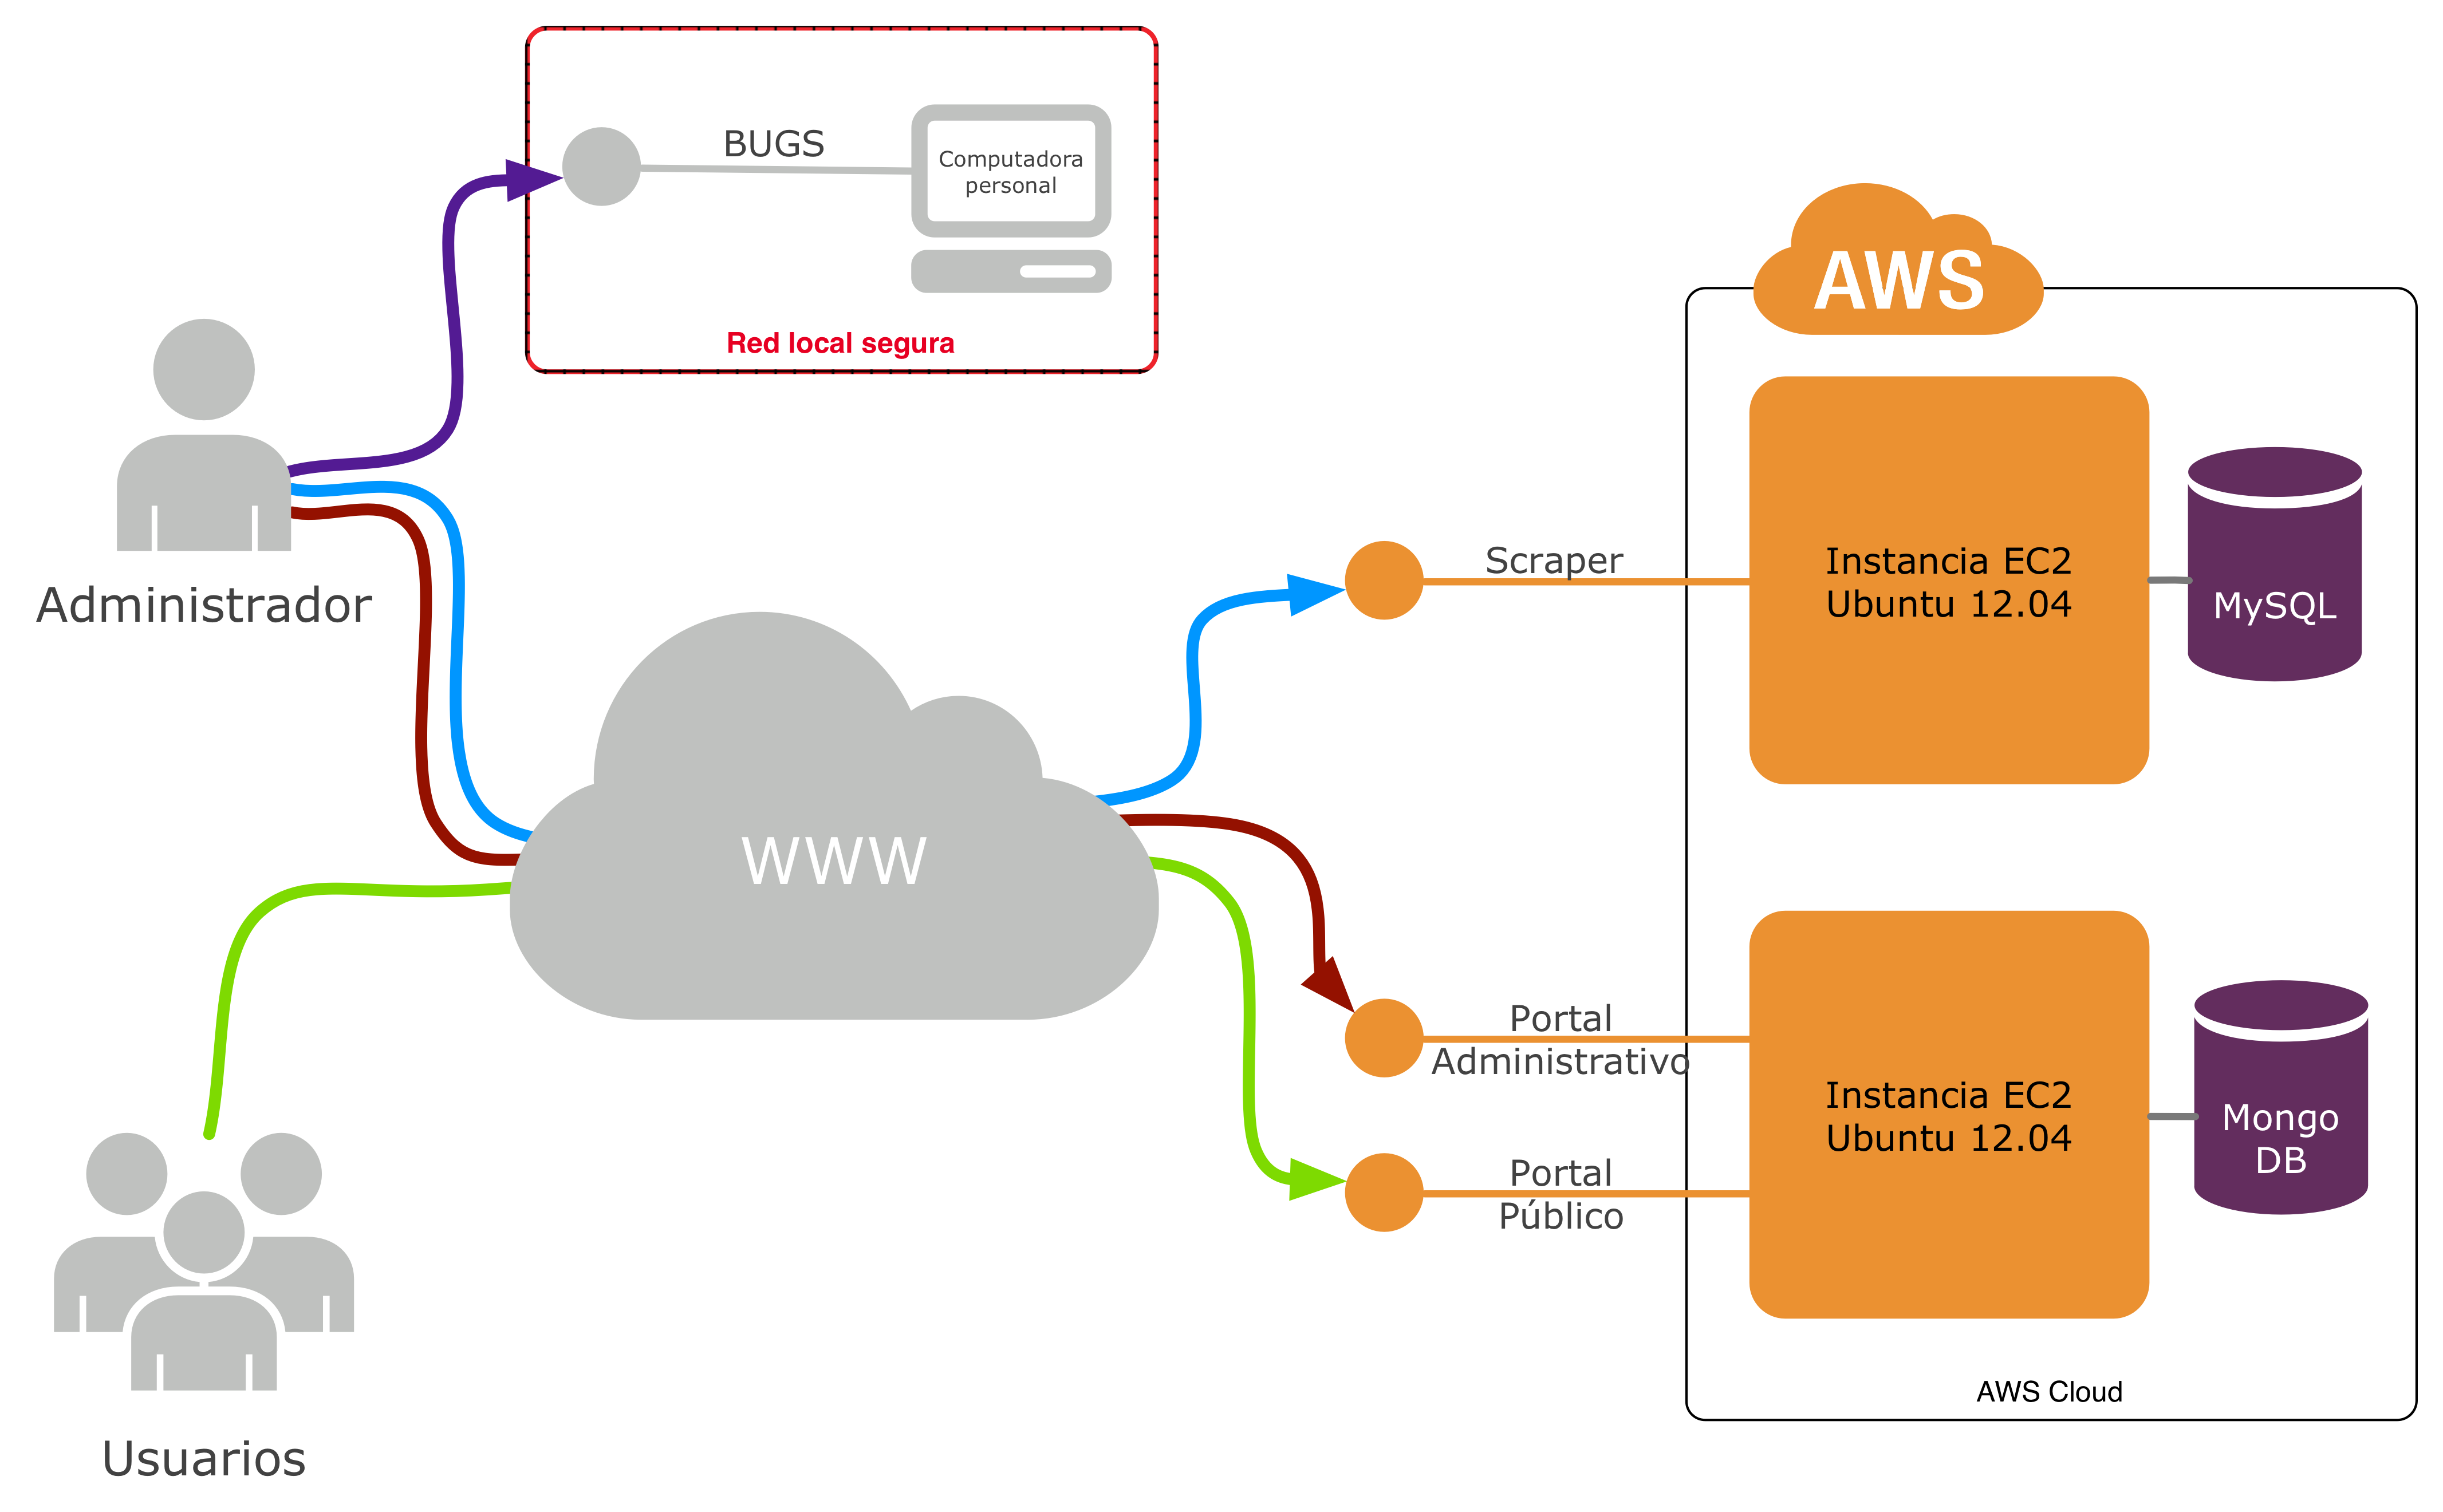
\includegraphics[width=\linewidth]{sistemas}
     \caption{Diagrama de sistemas y usuarios}\label{Fig:Sistemas}
   \end{minipage}
\end{figure}

El Sistema de recopilación de información y estadísiticas de los partidos (\emph{Sistema de recopilación}), el \emph{Portal administrativo} y el \emph{Portal público} corren bajo una arquitectura cliente servidor; mientras que el Sistema de estimación de probabilidades (\emph{Sistema de estimación}) corre en un ordenador personal.

Grosso modo el proceso que se lleva a cabo en el \emph{Back Office} para alimentar el \emph{Portal público} (Ver la figura~\ref{Fig:flujo}), se puede describir de la siguiente manera:
\begin{enumerate}
	\item A través del \emph{Sistema de recopilación} los administradores descargan de la página de Internet de ESPN los resultados de todos los partidos de la temporada junto con la información de los próximos partidos por jugar  de cada una de las ligas Europeas.
	\item Los datos recopilados permiten a los administradores generar un conjunto de archivos de texto con toda la información de los resultados de los últimos partidos y las fechas de los próximos partidos.
	\item Los administradores usan estos archivos para alimentar el \emph{Sistema de estimación} y calcular los pronósticos de los próximos partidos y las probabilidades de los resultados.
	\item Se obtienen los archivos que contienen la información de los próximos partidos así como la información de los equipos por liga y su desempeño en la temporada en curso.
	\item En el \emph{Portal administrativo} se ingestan los archivos obtenidos con la información de los próximos partidos, resultados de partidos anteriores y las estadísticas de los equipos en la temporada en curso.
	\item Finalmente, con la nueva información ingresada, los usuarios podrán disfrutar en el \emph{Portal público} sus recomendaciones peronalizadas de apuestas.
\end{enumerate}

\begin{figure}[!htb]\centering
   \begin {minipage}{1\textwidth}
     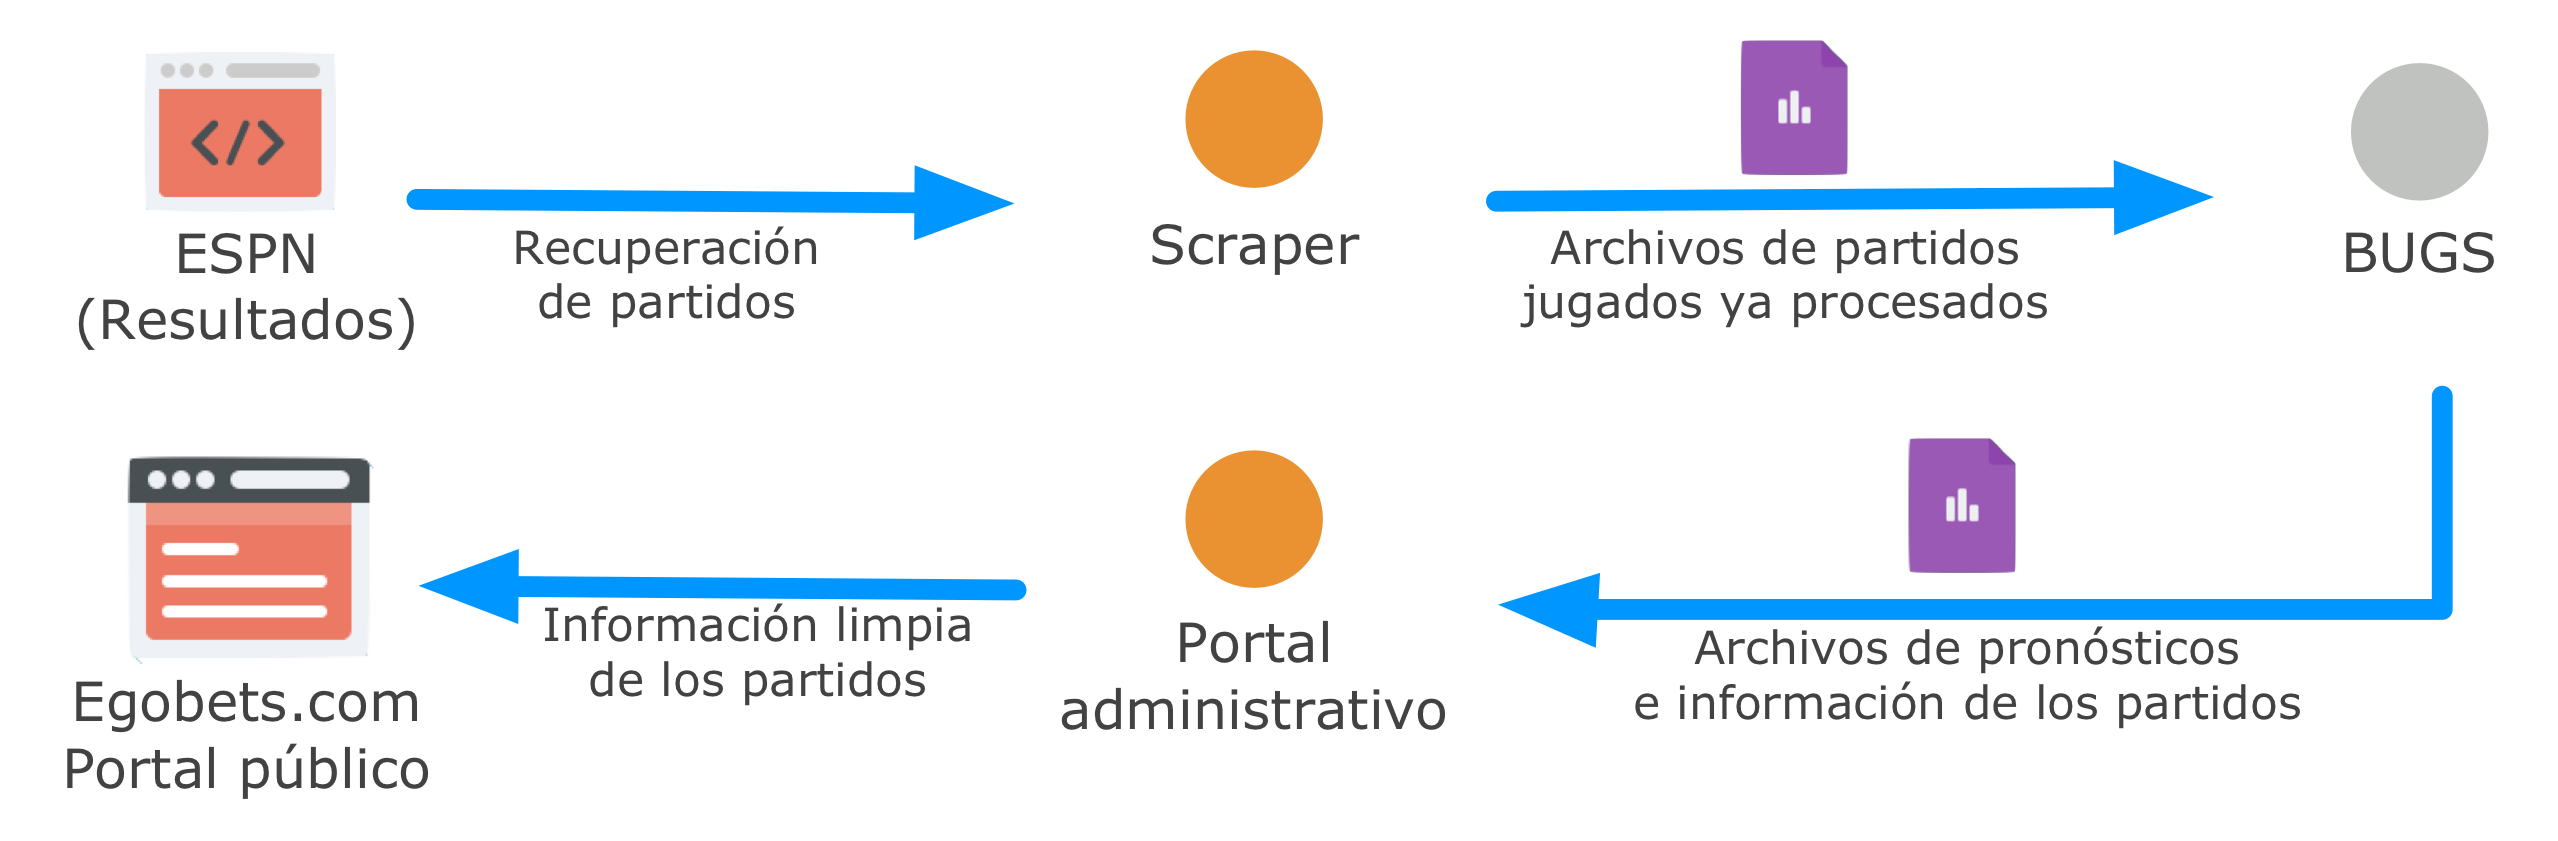
\includegraphics[width=\linewidth]{flujo}
     \caption{Diagrama de flujo de información}\label{Fig:flujo}
   \end{minipage}
\end{figure}


\section{Sistema de recopilación de información y estadísticas de los partidos}
\graphicspath{{/Users/brunomedina/Dropbox/Tesis-Egobets/egobets-notas/resources/recopilador/}}

A grandes rasgos el sistema de recopilación recupera todos los partidos que se juegan por temporada en cada una de las ligas\footnote{Egobets se enfoca en las ligas: alemana, españona, francesa, inglesa e italiana}. Para esto se dividirá este Sistema en los siguientes módulos:

\begin{enumerate}
	\item Recuperación de fechas de partidos próximos.
	\item Recuperación de información de partidos jugados.
	\item Generación de archivos con resultados.
\end{enumerate}


Adicionalmente en esta sección se describirá el funcionamiento del Sistema de Estimación. Sin embargo, al ser un conjunto de programas en \emph{Fortran} que son ajenos al autor, no se profundizará en los detalles del desarrollo del mismo.

Para poder comenzar la recuperación de información, es importante contar con los equipos que estén jugando esta temporada. Dependiendo de los resultados de la temporada anterior, los equipos que hayan quedado hasta abajo en la tabla de posición descienden a ligas menores y a su vez suben los mejores de estas ligas. Ver figura~\ref{Fig:los-equipos}

Al ingresar al \emph{Sistema de recopilación} se tienen 
\subsection{Diseño de la solución}
 \cite{alfredo2005ingenieria}


\begin{figure}[!htb]\centering
   \begin {minipage}{1\textwidth}
     \frame{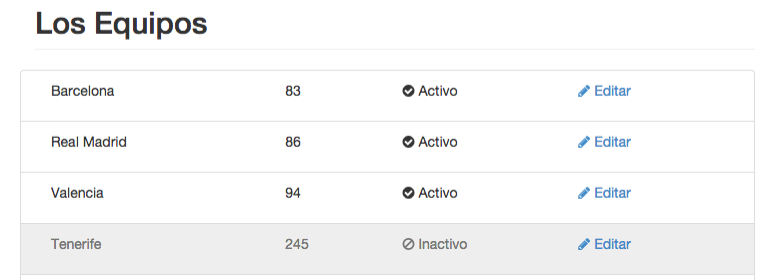
\includegraphics[width=\linewidth]{los-equipos}}
     \caption[Ejemplo de equipos de la liga española]{Ejemplo de equipos de la liga española\footnotemark }\label{Fig:los-equipos}
   \end{minipage}
\end{figure}

\footnotetext{Es importante mencionar que se usan aproximadamente los últimos quinientos partidos para la generación de los archivos, esto implica que se deben tener en base de datos los equipos que participaron en las pasadas dos temporadas de juegos. Por este motivo de pueden encontrar equipos que se encuentran en el sistema con la bandera de inactivos.}

\subsection{Recuperación de fechas de partidos próximos.}

\begin{figure}[!htb]\centering
   \begin {minipage}{1\textwidth}
     \frame{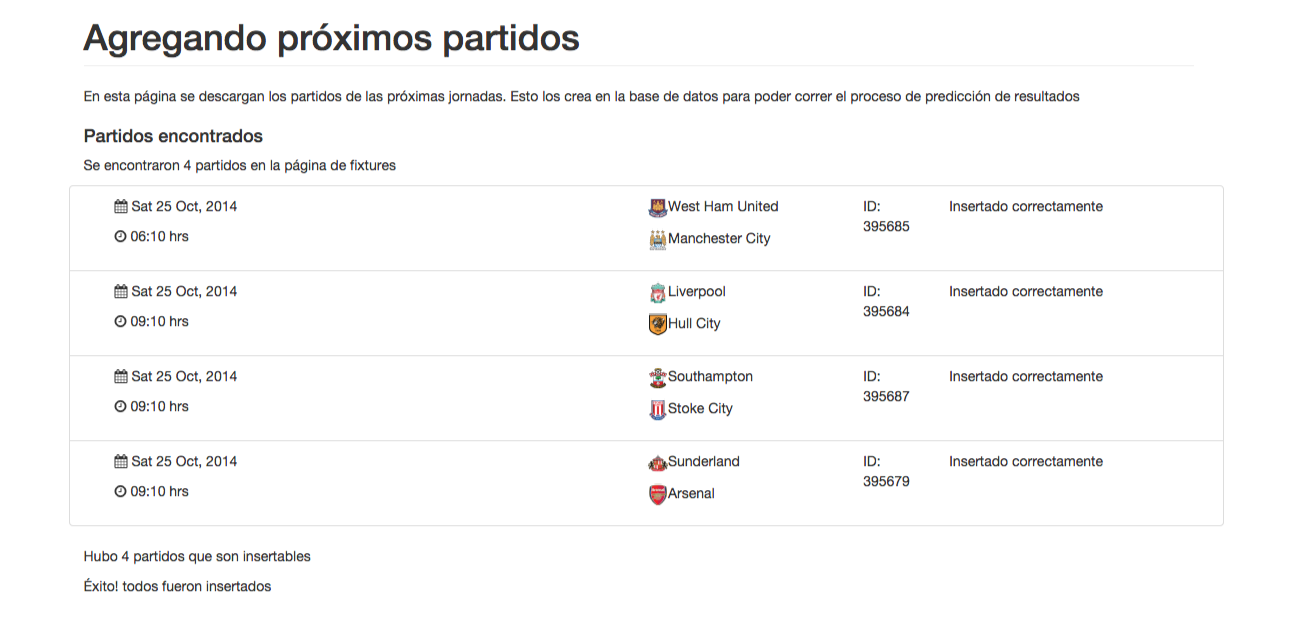
\includegraphics[width=\linewidth]{proximos-partidos}}
     \caption{Recuperación de próximos partidos}\label{Fig:proximos-partidos}
   \end{minipage}
\end{figure}

\subsection{Recuperación de información de partidos jugados.}

\begin{figure}[!htb]\centering
   \begin {minipage}{1\textwidth}
     \frame{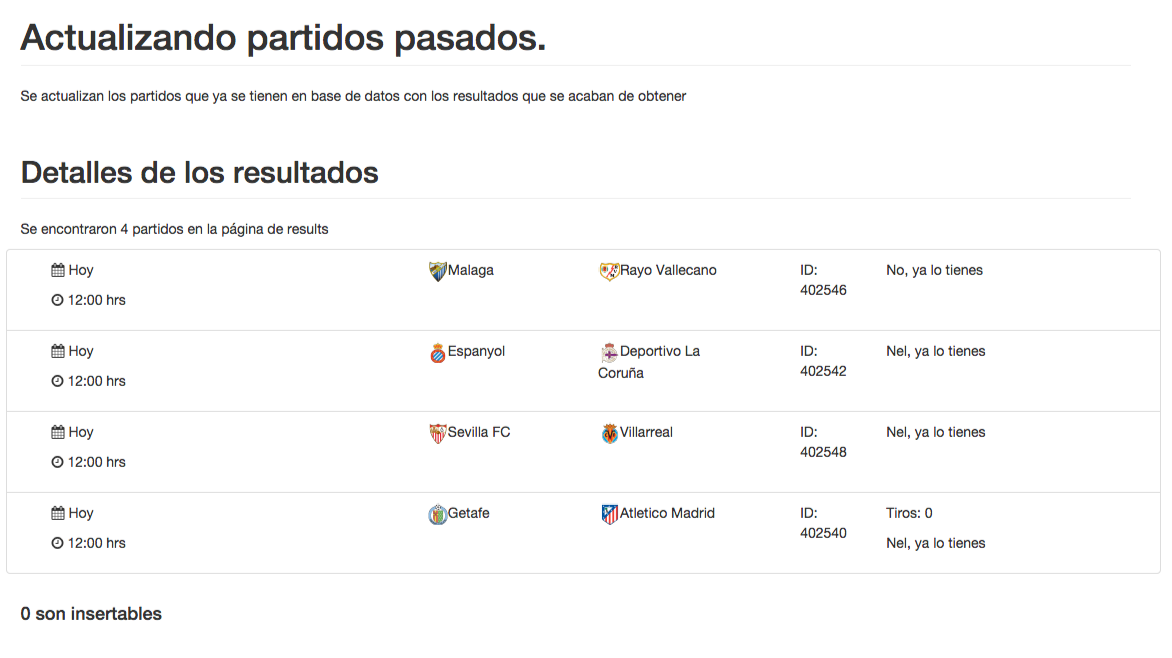
\includegraphics[width=\linewidth]{pasados-partidos}}
     \caption{Recuperación de resultados de partidos ya jugados}\label{Fig:pasados-partidos}
   \end{minipage}
\end{figure}

\subsection{Generación de archivos con resultados.}


\subsection{Sistema de estimación de probabilidades}
\section{Portal administrativo}
\graphicspath{{/Users/brunomedina/Dropbox/Tesis-Egobets/egobets-notas/resources/admin/}}

\subsection{Inicio de Sesión}
Se ingresa al sistema a través la dirección de internet: 
\begin{tightcenter}
	\textbf{https://admin.egobets.com}
\end{tightcenter}Se presenta la pantalla de inicio de sesión donde se introcue el nombre de usuario y contraseña. Véase las figuras~\ref{Fig:Login1} y~\ref{Fig:Login2}
\pagebreak
\begin{figure}[!htb]\centering
   \begin{minipage}{0.49\textwidth}
     \frame{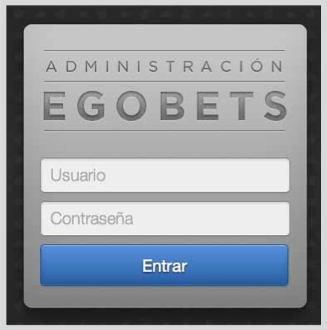
\includegraphics[width=\linewidth]{login}}
     \caption{Login}\label{Fig:Login1}
   \end{minipage}
   \begin {minipage}{0.49\textwidth}
     \frame{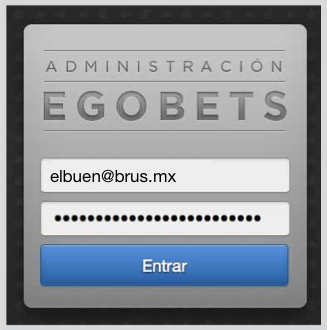
\includegraphics[width=\linewidth]{login-lleno}}
     \caption{Ingreso de datos}\label{Fig:Login2}
   \end{minipage}
\end{figure}

Al dar click en el botón de \underline{Entrar}, se habrá iniciado sesión, y se está habilitado para comenzar a trabajar.

Una vez que se haya terminado de usar el sistema, se debe cerrar la sesión, lo cual se puede hacer dando click sobre el botón de Salir. Véase figura~\ref{Fig:Logout}

\begin{figure}[!htb]\centering
   \begin {minipage}{0.49\textwidth}
     \frame{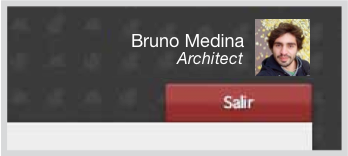
\includegraphics[width=\linewidth]{logout}}
     \caption[Cerrar Sesión]{Cerrar Sesión}\label{Fig:Logout}
   \end{minipage}
\end{figure}

Al hacerlo, se terminará de manera segura la sesión .
\subsection{Ingesta}
A través de este módulo se alimenta el sistema con la información necesaria para que la aplicación trabaje correctamente.

Lo elementos que se ingresan en este módulo son:

\begin{itemize}
\item Próximos partidos
\item Resultados de partidos anteriores
\item Estadísticas de los equipos en la temporada
\end{itemize}

Al entrar a esta sección, se encuentra un campo para seleccionar el tipo de ingesta que se quiere realizar, en este caso hay dos opciones:

\begin{itemize}
\item Partidos  
\item Equipos
\end{itemize}
Véase figura~\ref{Fig:ingesta}

\begin{figure}[!htb]\centering
   \begin {minipage}{0.8\textwidth}
     \frame{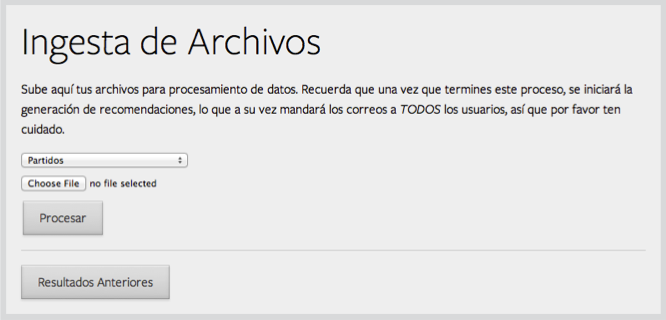
\includegraphics[width=\linewidth]{ingesta}}
     \caption[Subir y procesar archivos]{Subir archivos y procesarlos\footnotemark}
	 \label{Fig:ingesta}
   \end{minipage}
\end{figure}
\footnotetext{Toda la información referente a los archivos que se deben subir se encuentra en el~\cref{chap:archivos} }




\subsubsection{Partidos}
\begin{figure}[!htb]\centering
   \begin {minipage}{1\textwidth}
     \frame{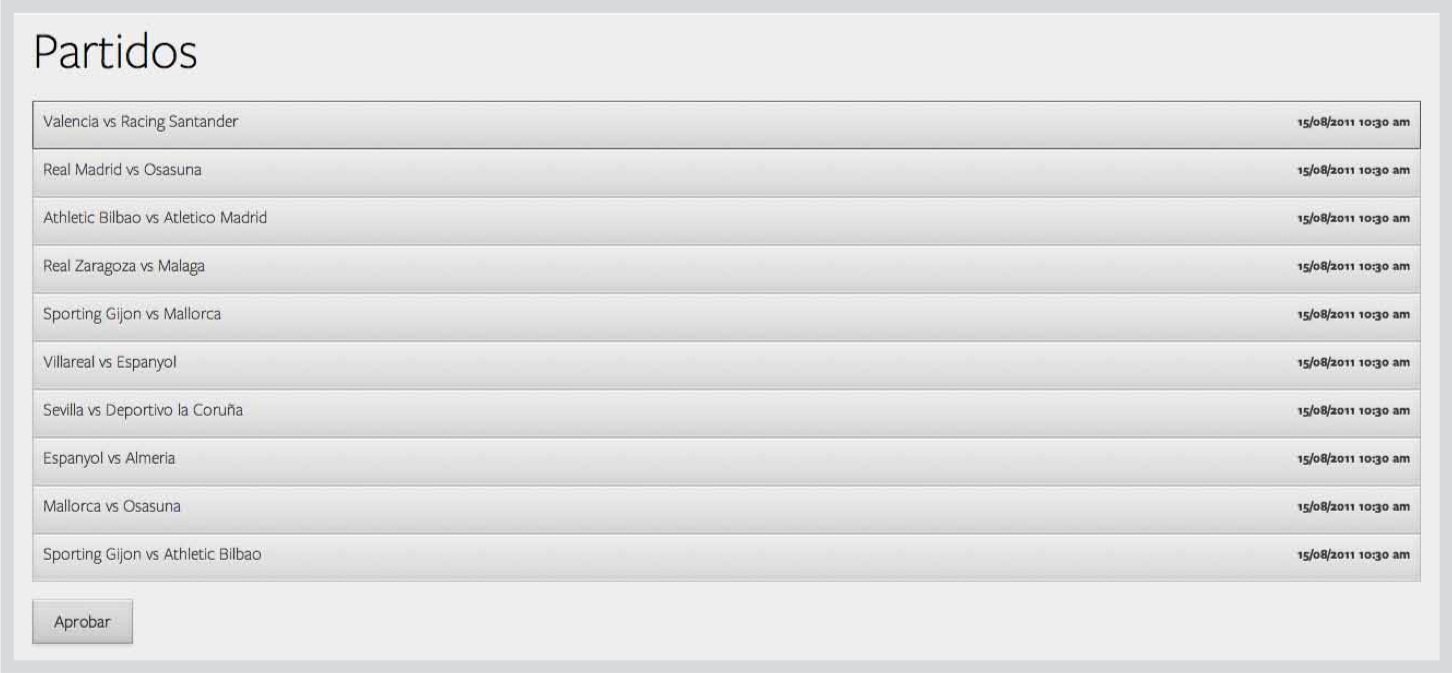
\includegraphics[width=\linewidth]{partidos}}
     \caption{Partidos procesados por el sistema}
	 \label{Fig:partidos}
   \end{minipage}
\end{figure}

Para subir la información de los partidos de la jornada que comienza, se selecciona del menú la opción de \textbf{Partidos}, y se presiona el botón \underline{Seleccionar archivo} donde se elige el archivo correspondiente.
Una vez seleccionado el archivo a ingestar y el tipo de datos que contiene, se oprime el botón de \underline{Procesar}, lo cual comienza el proceso de ingesta.\footnote{Una vez que comenzado el proceso de ingesta (ya sea de equipos ó partidos), se tienen sólo 10 minutos para verificar que los datos sean correctos. De no hacerlo, el sistema no procesará el archivo hasta que se suba nuevamente}

Con el archivo ya procesado, se puede verificar la interpretación que el sistema realizó del archivo. Se pueden observar en pantalla los siguientes datos:
\begin{itemize}
\item Identificador único y nombre del equipo local
\item Identificador único y nombre del equipo visitante
\item Marcadores de equipo local y visitante
\item Probabilidades de local, empate y visitante
\item Fecha en la que se llevará a cabo el partido
\end{itemize}

Si hay algún error en la información se puede presionar \underline{Cancelar} e intentarlo nuevamente, si la información es la correcta se oprime el botón de \underline{Aceptar}.


\subsubsection{Equipos}
\begin{figure}[!htb]\centering
   \begin {minipage}{1\textwidth}
     \frame{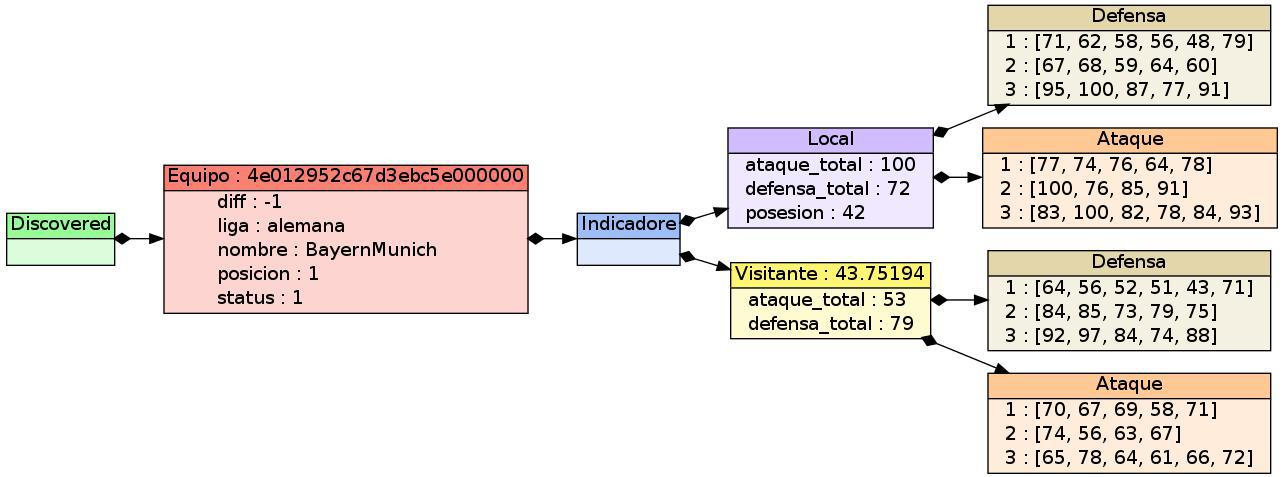
\includegraphics[width=\linewidth]{equipos}}
     \caption{Actualizando datos de los equipos}
	 \label{Fig:equipos}
   \end{minipage}
\end{figure}

Para la ingesta de datos de los equipos se selecciona la pestaña de \underline{Equipos} en la pestaña y luego se presiona el botón \textbf{Seleccionar archivo}.
Una vez que se seleccione el archivo a ingestar y el tipo de datos que contiene, se oprime el botón de \underline{Procesar}, para comenzar el proceso de ingesta.
Cuando el archivo termina de ser procesado el sistema presentará la interpretación del archivo, donde se podrán verificar los siguientes datos:
\begin{itemize}
\item Nombre del equipo
\item Indicadores de ataque y promedio de ataques:
	\begin{itemize}
		\item Medio Centro
		\item Delanteros
		\item Definición
	\end{itemize}
\item Indicadores de defensa y promedio de defensas:
	\begin{itemize}
		\item Medio centro,
		\item Defensa
		\item Portero
		\item Posesión
	\end{itemize}
\end{itemize}

Si hay algún error en la información se puede presionar \underline{Cancelar} e intentarlo nuevamente, si la información es la correcta se oprime el botón de \underline{Aceptar}.


\subsubsection{Resultados Anteriores}

Al dar clic en el botón de \underline{Resultados Anteriores} se pueden ver y modificar los resultados de los partidos de la semana pasada. En esta pantalla se actualizan los marcadores, al terminar se da click en \underline{Guardar Resultados}.

\begin{figure}[!htb]\centering
   \begin {minipage}{0.64\textwidth}
     \frame{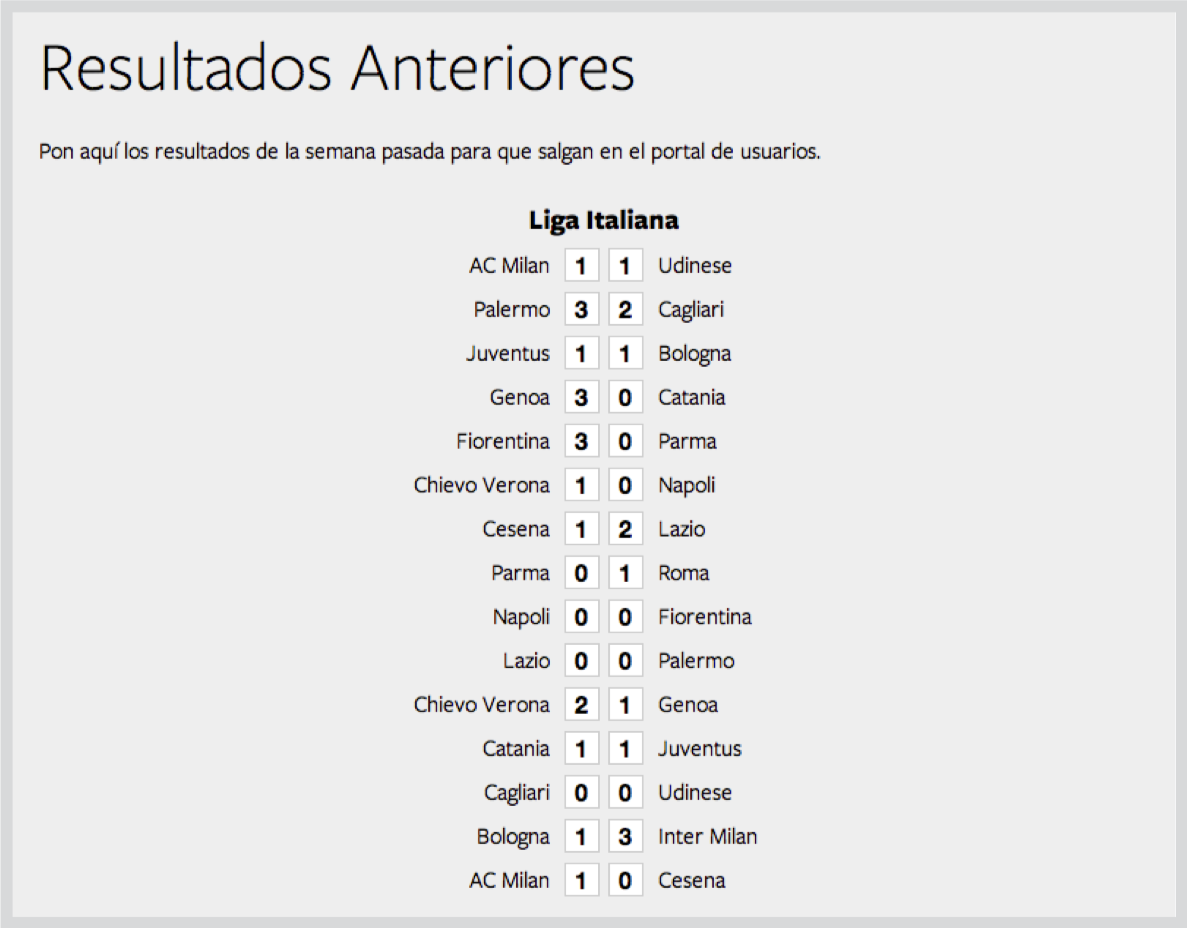
\includegraphics[width=\linewidth]{resultados-anteriores}}
     \caption[Actualizar resultados Anteriores]{Actualizando marcadores de la liga italiana}
	 \label{Fig:Resultados-anteriores}
   \end{minipage}
\end{figure}

Si el marcador de un partido que ya tenía resultado se deja en blanco no será modificado al guardar y se mostrará el resultado que tenía previamente.

\subsection{Usuarios}

Se muestran de quince en quince todos los usuarios inscritos a Egobets, para ver los siguientes quince usuarios se da click en el botón \underline{Siguiente}. Cada usuario tiene un botón de \underline{Detalles} y \underline{Eliminar}.
\begin{figure}[!htb]\centering
   \begin {minipage}{1\textwidth}
     \frame{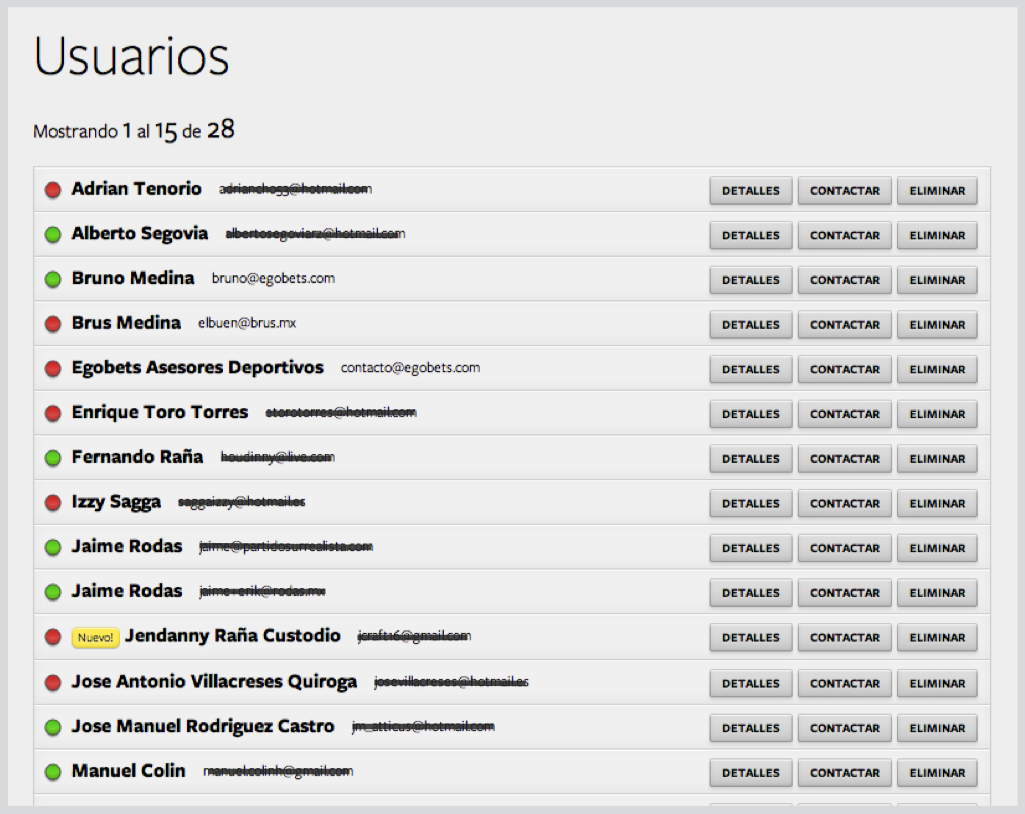
\includegraphics[width=\linewidth]{usuarios}}
     \caption{Listado de Usuarios}
	 \label{Fig:usuarios}
   \end{minipage}
\end{figure}

\subsubsection{Detalles de Usuario}

El botón Detalles en el listado presenta la información más detallada del usuario. Aquí se puede ver su información y preferencias:

\begin{figure}[!htb]\centering
   \begin {minipage}{1\textwidth}
     \frame{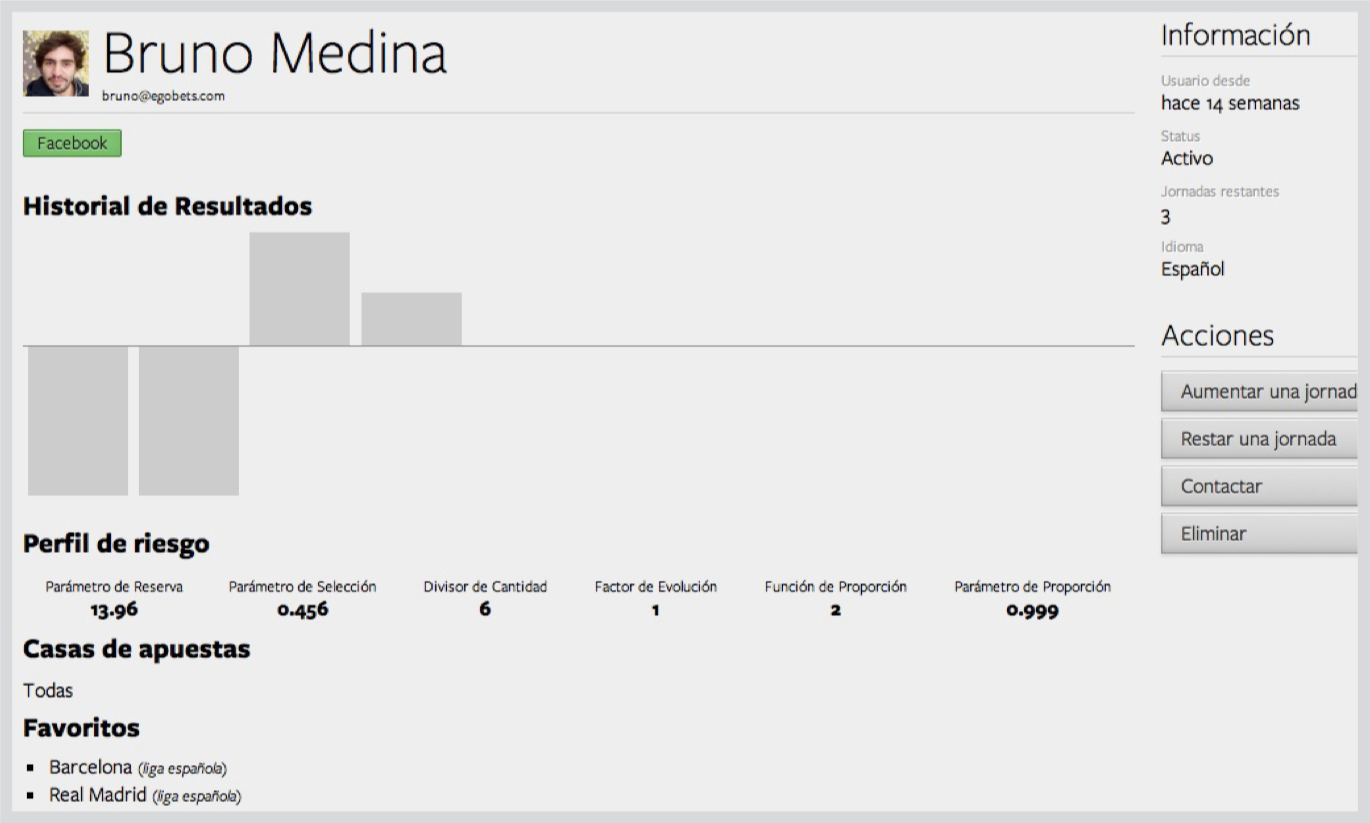
\includegraphics[width=\linewidth]{detalle-usuario}}
     \caption{Vista del detalle de usuario}
	 \label{Fig:Detalle-usuario}
   \end{minipage}
\end{figure}

\begin{itemize}
	\item \textbf{Historial.} Indica las últimas ganancias y pérdidas por jornada
	\item \textbf{Perfil de riesgo.} Despendiendo de la encuesta realizada por usuario se tiene su adversidad al riesgo.
	\item \textbf{Casas de apuesta.} En el sistema se tienen varias Casas que proporcionan distintos momios para los partidos.
	\item \textbf{Favoritos.} Los equipos favoritos del usuario
	\item \textbf{Transacciones realizadas.} Los últimos pagos realizados.
	\item \textbf{Usuario desde.} Tiempo que lleva como usuario de Egobets.
	\item \textbf{Estatus de actividad.} Al ser un sistema de paga los usuarios pagan por jornada para recibir la asesoría de apuestas.
		\begin{itemize}
			\item Activo: el usuarios está recibiendo recomendaciones.
			\item Inactivo: el usuario no está recibiendo recomendaciones.
		\end{itemize}
	\item \textbf{Jornadas restantes.} La cantidad de Jornadas que el usuario va seguir recibiendo asesorías.
	\item \textbf{Idioma.} En que lenguaje lee el portal el usuario (Inglés o Español)
\end{itemize}

\textbf{Acciones Administrativas}
\begin{itemize}
\item \textbf{Aumentar/Restar una Jornada.}
Una jornada le permite al usuario recibir la asesoría de los siguientes partidos.
Los administradores del sistema le pueden otorgar o quitar a los usuarios jornadas con tan solo click en el botón.

\item \textbf{Contactar.}
Permite al administrador enviar un correo desde su progama predeterminado de correo al usuario.

\item \textbf{Eliminar.} Todos los datos del usuario son eliminados del sistema.
\end{itemize}

\begin{figure}[!htb]\centering
   \begin {minipage}{0.5\textwidth}
     \frame{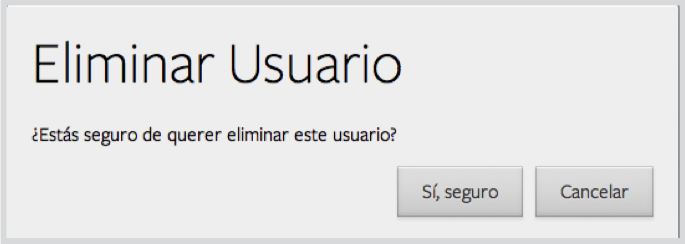
\includegraphics[width=\linewidth]{eliminar-usuario}}
     \caption[Confirmar la eliminación de un usuario]{Confirmar la eliminación de un usuario\footnotemark}
	 \label{Fig:Eliminar-usuario}
   \end{minipage}
\end{figure}

\footnotetext{La información de los usuarios eliminados no podrá ser rescatada.}

\subsection{Pagos}
Los pagos de los usuarios se cambian por la sugerencia de apuestas de una jornada. En esta sección se muestra un listado de las transacciones monetarias más recientes y su información general.

\begin{figure}[!htb]\centering
   \begin {minipage}{1\textwidth}
     \frame{\includegraphics[width=\linewidth]{Transacciones}}
     \caption{Listado con los últimos pagos realizados}
	 \label{Fig:Transacciones}
   \end{minipage}
\end{figure}

Los detalles de las transacciones son:
\begin{itemize}
	\item Fecha en la que la transacción se inicio.
	\item Número de transacción en la cuenta de PayPal de Egobets.
	\item Nombre y el correo del usuario que realiza la transacción, al dar clic sobre su nombre serán dirigidos a la información detallada de dicho usuario
	\item Cantidad de jornadas por las que se realiza la transacción
	\item Cantidad monetaria por la que se realiza la transacción
	\item Estatus de la transacción:
	\begin{itemize}
		\item Pendiente: se ha iniciado la transacción para la compra de jornadas, sin embargo aun no ha concluido.
		\item Pagada: se realizó exitosamente y las jornadas han sido agregadas al usuario.
	\end{itemize}
\end{itemize}

\subsection{Estadísticas}

Esta sección muestra las estadísticas y gráficas a los usuarios administrativos con información relevante de: ganancias y pérdidas de los usuarios, resultados de las predicciones, preferencias de los usuarios, pagos y partidos.

\subsubsection{Resultados Netos}

Indica el promedio de las ganancias y pérdidas de todos los usuarios en las últimas cinco jornadas, esta información se puede ver de manera porcentual o en cantidad neta.
Véase figura~\ref{Fig:mayor-ganancia}
\begin{figure}[!htb]\centering
   \begin {minipage}{0.4\textwidth}
     \frame{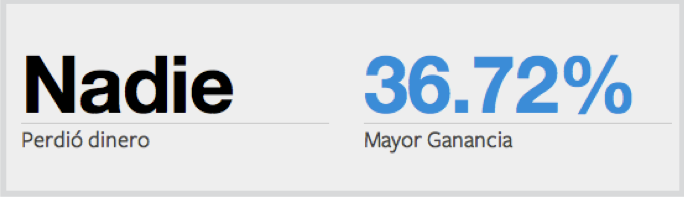
\includegraphics[width=\linewidth]{mayor-ganancia}}
     \caption{Ganancias y pérdidas de los usuarios}
	 \label{Fig:mayor-ganancia}
   \end{minipage}
\end{figure}


\textbf{Mayor Pérdida.}
Indica la mayor pérdida porcentual que se ha dado en la última jornada y al dar click presenta el perfil de dicho usuario.

\textbf{Mayor Ganancia.}
Indica la ganancia porcentual mayor que se ha dado en la última jornada y al dar click presenta el perfil de dicho usuario.


\subsubsection{Usuarios y sus Datos}

\textbf{Total.} Número total de usuarios registrados y al dar click presenta la sección de \underline{Usuarios}.

\textbf{Nuevos.} Número de usuarios registrados recientemente y al dar click presenta la sección de \underline{Usuarios}.

Véase figura~\ref{Fig:nuevos-usuarios}
\begin{figure}[!htb]\centering
   \begin {minipage}{0.4\textwidth}
     \frame{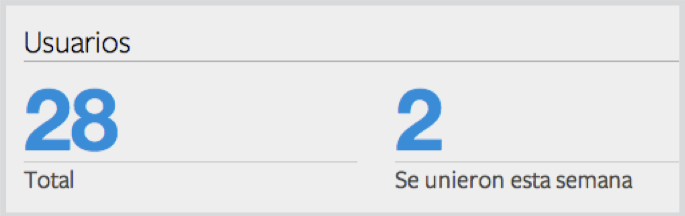
\includegraphics[width=\linewidth]{nuevos-usuarios}}
     \caption{Usuarios recién inscritos}
	 \label{Fig:nuevos-usuarios}
   \end{minipage}
\end{figure}

Además, el sistema muestra la siguiente información general, porcentaje de usuarios que:
\begin{itemize}
	\item Usan Facebook para conectarse a Egobets
	\item Usan apuestas dobles
	\item Usan reserva
	\item Ven Egobets en inglés
	\item Se encuentran activos.
\end{itemize}
Véase figura~\ref{Fig:graficas-usuarios}
\begin{figure}[!htb]\centering
   \begin {minipage}{1\textwidth}
     \frame{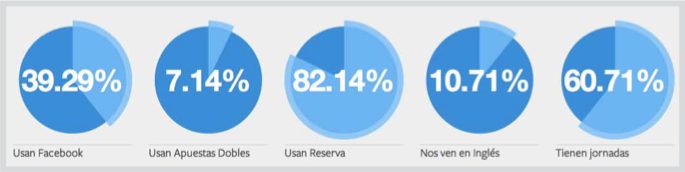
\includegraphics[width=\linewidth]{graficas-usuarios}}
     \caption{Datos estadísticos de los usuarios}
	 \label{Fig:graficas-usuarios}
   \end{minipage}
\end{figure}
 
\subsubsection{Pagos Recibidos}

\begin{figure}[!htb]\centering
   \begin {minipage}{0.5\textwidth}
     \frame{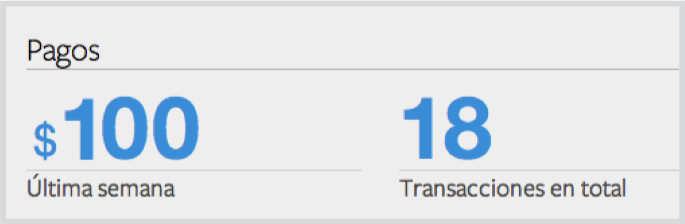
\includegraphics[width=\linewidth]{ultimos-pagos}}
     \caption{Pagos más recientes}
	 \label{Fig:ultimos-pagos}
   \end{minipage}
\end{figure}

\textbf{Última Semana.}
Se representan las ganancias monetarias que obtenidas durante la última semana. Al dar click se muestra la sección de \textbf{Pagos}.

\textbf{Transacciones en total.}
Indica el número de transacciones que se han realizado durante todo el tiempo del sistema.

\subsubsection{Partidos y Predicciones}

\begin{figure}[!htb]\centering
   \begin {minipage}{0.5\textwidth}
     \frame{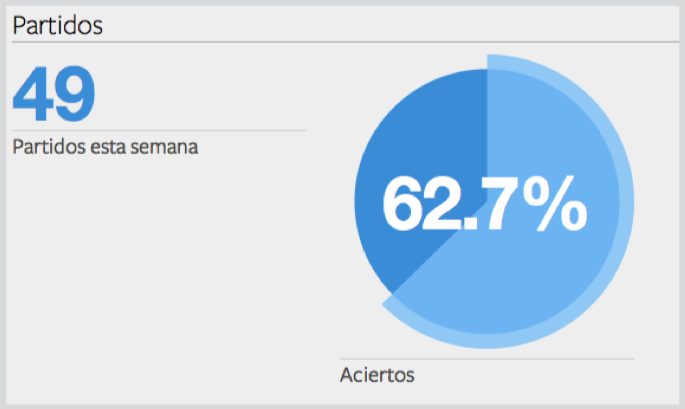
\includegraphics[width=\linewidth]{partidos-acertados}}
     \caption{Partidos acertados}
	 \label{Fig:partidos-acertados}
   \end{minipage}
\end{figure}

\textbf{Aciertos}
Presenta la cantidad de partidos de esta semana y al dar clic nos lleva a la sección de \underline{Ingesta}.

\textbf{Aciertos}
Representan con una gráfica la cantidad de aciertos obtenidos en las predicciones hechas en partidos pasados. Al presionarla se dirige el navegador a los \underline{Resultados Anteriores} dentro de la sección de \underline{Ingesta}.

\subsection{Correos}

En esta sección se puede enviar correos a un subconjunto de usuarios registrados en Egobets. Los mensajes deberán ser escritos en Español y en Inglés para que el correo recibido dependa del lenguaje elegido por el usuario al crear su cuenta. Los grupos de usuarios con los que nos se puede comunicar son:

\begin{itemize}
	\item Todos los usuarios
	\item Usuarios activos: aquellos que tienen jornadas pagadas
	\item Usuarios inactivos: aquellos que ya no tienen jornadas pagadas
	\item Usuarios registrados: aquellos que se registraron pero no han confirmado su correo
\end{itemize}
Véase figura~\ref{Fig:correos}

\begin{figure}[!htb]\centering
   \begin {minipage}{0.8\textwidth}
     \frame{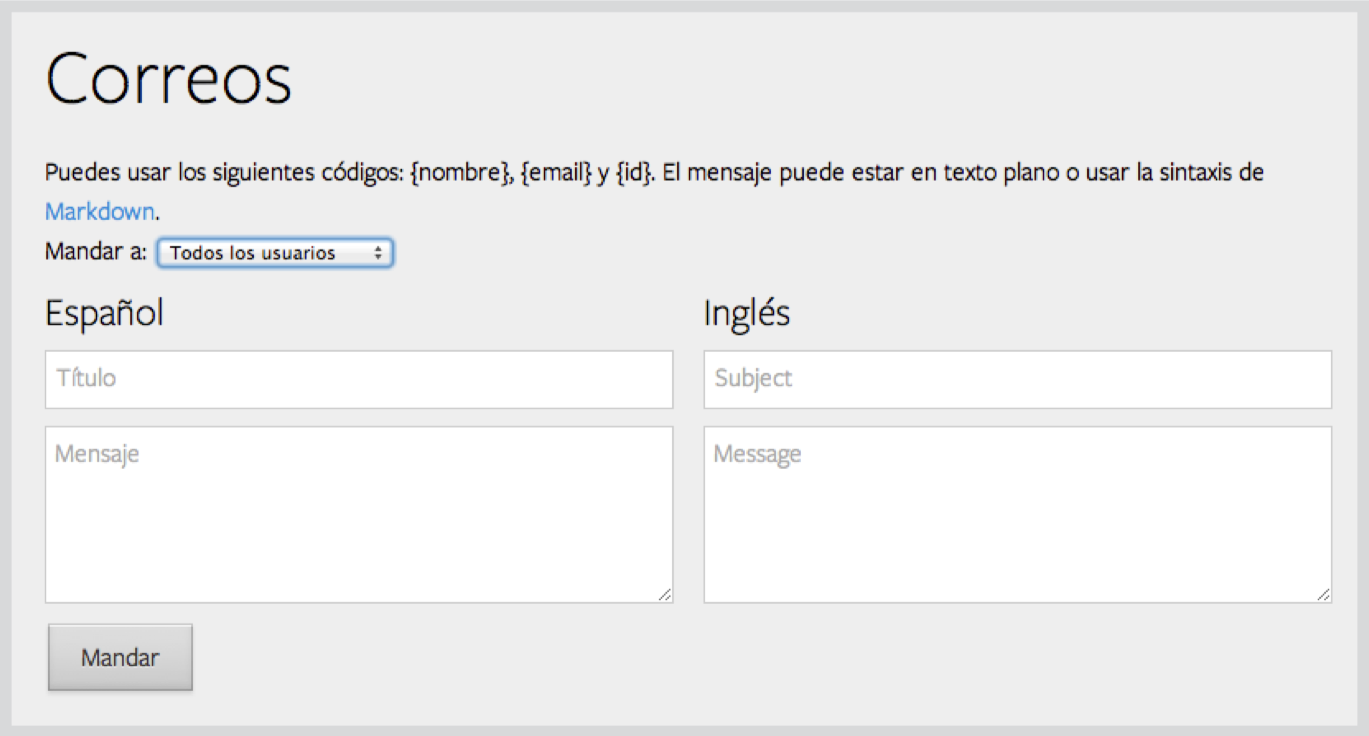
\includegraphics[width=\linewidth]{correos}}
     \caption{Comunicación con los usuarios}
	 \label{Fig:correos}
   \end{minipage}
\end{figure}

Para redactar los textos, se debe usar la sintaxis de Markdown\footnote{El hipervínculo de \underline{Markdown} redirige a una página dónde se puede aprender sobre el uso de esta sintaxis.}.
Se pueden usar textos de reemplazo cuándo se quieran personalizar los mensajes, para esto basta con utilizar las palabras clave: \{nombre\}, \{correo\} y \{id\}, las cuales el sistema sustituirá, al momento de mandar el correo, por los valores correspondientes para cada usuario.




